\chapter{Grafi e Approccio Multi-Livello}\label{ch:cap1}

In questo capitolo sono presentati alcuni concetti introduttivi utili alla definzione e alla comprensione dei
\textit{Grafi Multi-livello}.
Verr\`a esplorato il concetto fondamentale di grafo, una struttura matematica in grado di rappresentare relazioni tra
elementi discreti, e verranno illustrati i fondamenti della teoria dei grafi~\cite{cormen2010introduction,gross2018graph},
la disciplina che si occupa dello studio di queste strutture, utile in svariati ambiti applicativi, come l'informatica,
l'ingegneria, la biologia, la chimica ed altri.
Maggiore attenzione sar\`a rivolta alle definizioni pertinenti al partizionamento e alla contrazione di
grafi ~\cite{Sanders2012HighQG}, vicine alle caratteritiche salienti dei \textit{Grafi Multi-livello},
evidenziando gli aspetti gi\`a trattati nella letteratura esistente e quelli che verranno approfonditi in questa tesi.

\section{Cenni di Teoria dei Grafi}\label{sec:cenni-di-teoria-dei-grafi}

Un grafo \`e una struttura matematica costruita su un insieme di elementi in cui coppie di elementi possono essere
in relazione tra loro.
I grafi possono essere orientati o non orentati, a seconda che esista una direzione o un ordine tra le coppie
di elementi che si trovano in relazione.
In questa sezione ci concentreremo eclusivamente sui grafi diretti, in quanto pi\`u generali, visto che grafi
non orientati possono sempre essere rappresentati come particolari grafi orientati, ed in quanto la struttura dei
\textit{Grafi Multi-livello} si basa su di essi.

\subsection{Grafo Orientato}\label{subsec:grafo-orientato}

\begin{definition}[Grafo orientato]
    Un \textbf{grafo orientato} $G$ \`e una coppia $(V, E)$, dove:
    \begin{itemize}
        \item $V  = \{v_1, v_2, \ldots, v_n\}$ \`e un di un insieme finito non vuoto di elementi detti \textbf{nodi}
        (o \textbf{vertici}).
        \item $E = \{(v_i, v_j) \mid v_i, v_j \in V\} \subseteq V \times V$ \`e un insieme di coppie ordinate di
        nodi dette \textbf{archi} (o \textbf{spigoli}).
    \end{itemize}
\end{definition}

Nelle rappresentazioni grafiche dei grafi orientati, i nodi sono solitamente rappresentati
come cerchi o punti, mentre gli archi come frecce.
Nella figura~\ref{fig:directed-graph-example} \`e mostrato un esempio di grafo orientato con insieme di nodi
$V = \{v_1, v_2, v_3, v_4, v_5, v_6, v_7\}$ e insieme di archi $E = \{(v_1, v_2), (v_2, v_1), (v_2, v_3), (v_3, v_1)
(v_3, v_4), \\ (v_4, v_4), (v_5, v_6), (v_6, v_5)\}$. \newline
Si noti che sono ammessi \textbf{cappi}, ovvero archi che collegano un nodo a se stesso, ma nella normale nozione
di grafo orientato non sono ammessi archi multipli tra due nodi.

\begin{figure}[h]
    \centering
    \begin{tikzpicture}
    % Define the nodes
    \node[mynode] (1) at (0, 0) {$v_1$};
    \node[mynode] (2) at (2, 2) {$v_2$};
    \node[mynode] (3) at (4, 0) {$v_3$};
    \node[mynode] (4) at (2, -2) {$v_4$};
    \node[mynode] (5) at (6, 2) {$v_5$};
    \node[mynode] (6) at (8, 0) {$v_6$};
    \node[mynode] (7) at (6, -2) {$v_7$};

    % Draw the edges
    \draw[myarrow] (1) -- (2);
    \draw[myarrow] (2) to[out=180, in=90] (1);
    \draw[myarrow] (4) to[out=225, in=135, looseness=5] (4); % This edge is a self-loop, corrected below
    \draw[myarrow] (2) -- (3);
    \draw[myarrow] (3) -- (4);
    \draw[myarrow] (3) -- (1);
    \draw[myarrow] (5) to[out=0, in=90] (6);
    \draw[myarrow] (6) -- (5);
\end{tikzpicture}
    \caption{Un esempio di grafo orientato}
    \label{fig:directed-graph-example}
\end{figure}

Le cardintalit\`a degli insiemi di nodi e archi di un grafo orientato sono rispettivamente $|V| = n$ e $|E| = m$,
e vengono dette rispettivamente \textbf{ordine} e \textbf{dimensione} del grafo.

Essendo definiti su un insieme di elementi e di archi, possono essere definite relazioni di inclusione tra grafi.
Un grafo $G' = (V', E')$ \`e un sottografo di $G = (V, E)$, e lo si indica con $G' \subseteq G$ se $V' \subseteq V$
e $E' \subseteq E$. \newline
Inoltre, dato un certo insieme $V' \subseteq V$, si definisce il sottografo di $G$ \textbf{indotto} da $V'$, e lo si
indica con la notazione $G[V']$, il grafo avente come insieme di nodi $V'$ e come insieme di archi l'insieme di tutti
gli archi in $G$ che rappresentino relazioni tra tali nodi, ovvero il grafo $G' = (V', E')$ dove
$E' = \{ (u, v) \in E : u, v \in V'\}$. \newline

Essendo il contenuto informativo rilevante di un grafo orientato contenuto nei suoi archi, e quindi nelle relazioni
tra nodi, il concetto di eguaglianza tra grafi orientati non \`e banale.
Una relazione tra grafi orientati, utile per valutare la loro equivalenza in termini di informazione espressa,
\`e l'isomorfismo (dal greco \textit{iso} = uguale e \textit{morph\`e} = forma).
Cos\`{\i} come per tutte le struttre matematiche, intuitivamente, due grafi si dicono \textbf{isomorfi} quando per ogni
parte della struttura di uno esiste una corrispondente parte della struttura dell'altro, e viceversa.
Formalmente, due grafi orientati $G = (V, E)$ e $H = (W, F)$ si dicono isomorfi, e lo si indica con $G \cong H$ se
esiste una biiezione $f: V \rightarrow W$ tale per cui $(u, v) \in E$ se e solo se $(f(u), f(v)) \in F$ per ogni
$u, v \in V$. \newline

\subsection{Archi e nodi}\label{subsec:archi-e-nodi-di-un-grafo-orientato}

A seguire alcune definizioni relative ai nodi e agli archi di un grafo orientato: \newline

Sia $(u, v) \in E$ un arco di un grafo orientato $G = (V, E)$, allora:
\begin{itemize}
    \item l'arco $(u, v)$ \textbf{esce} dal nodo $u$ ed {entra} nel nodo $v$.
        Ad esempio, gli archi uscenti dal nodo $v_2$ nel grafo della figura~\ref{fig:directed-graph-example}
        sono $(v_2, v_1)$ e $(v_2, v_3)$, mentre l'unico arco entrante nel nodo $v_5$ \`e $(v_6, v_5)$.
    \item l'arco $(u, v)$ si dice \textbf{incidente} in entrambi i vertici $u$ e $v$.
    \item il nodo $v$ \`e detto \textbf{adiacente} al nodo $u$, in quanto esiste un arco $(u, v) \in E$.
\end{itemize}

Sia $v \in V$ un nodo di un grafo orientato $G = (V, E)$, allora:
\begin{itemize}
    \item il \textbf{grado uscente} di un nodo $v$ \`e il numero di archi che escono da $v$.
    \item il \textbf{grado entrante} di un nodo $v$ \`e il numero di archi che entrano in $v$.
    \item il \textbf{grado} di un nodo $v$ \`e la somma del grado uscente e del grado entrante di $v$.
\end{itemize}

\subsection{Cammini}\label{subsec:cammini}

I cammini sono concetti fondamentali della teoria dei grafi e sono alla base di molti algoritmi e problemi noti
relativi ai grafi. \newline

Sia $G = (V, E)$ un grafo orientato, siano $u, v \in V$ due nodi di $G$, allora un \textbf{cammino} da $u$ a $v$ in $G$
\`e una sequenza ordinata di nodi $\langle v_0, v_1, \ldots, v_k \rangle$ tale che $(v_i, v_{i+1}) \in E$ per ogni
$i = 0, 1, \ldots, k-1$ con $v_1 = u$ e $v_k = v$.
La \textbf{lunghezza} k di un cammino \`e data dal numero di archi che lo compongono.
Ad esempio, $\langle v_1, v_2, v_3, v_4 \rangle$ \`e un cammino di lunghezza 3 nel grafo della
figura~\ref{fig:directed-graph-example}. \newline

Se esiste un cammino $p$ da $u$ a $v$ in $G$, allora si dice che il nodo $v$ \`e \textbf{raggiungibile} da $u$
attraverso $p$ in $G$, e questo pu\`o essere indicato con la notazione $u \overset{p}{\rightsquigarrow} v$. \newline

A seguire alcune definizioni relative ai cammini su un grafo orientato:

\begin{itemize}
    \item Un cammino si dice \textbf{semplice} se non contiene nodi ripetuti, ad eventuale eccezione del primo e
    dell'ultimo nodo.
    \item Un cammino si dice \textbf{elementare} se non contiene archi ripetuti. Si noti che un cammino semplice \`e
    sempre elementare.
    \item Un cammino $\langle v_0, v_1, \ldots, v_k \rangle$ di lunghezza $k \geq 1$ si dice \textbf{ciclo} se $v_1 = v_k$, ovvero se il
    suo nodo iniziale coincide con il suo nodo finale.
    Un \textbf{ciclo semplice} \`e un cammino in cui tutti i nodi sono distinti, ad eccezione del primo e dell'ultimo
    nodo, mentre un \textbf{ciclo elementare} (o \textbf{circuito}) \`e un ciclo in cui tutti gli archi sono distinti.
    Ad esempio, nel grafo in figura~\ref{fig:directed-graph-example}, il cammino $\langle v_1, v_2, v_3, v_1 \rangle$
    \`e un circuito semplice di lunghezza 3.
    Inoltre, un grafo diretto che non contiene cicli semplici \`e detto grafo diretto \textbf{aciciclico} (o
    \textbf{DAG}).
    \item Un cammino si dice \textbf{cammino hemiltoniano} in nel grafo $G$ se attraversa ogni nodo di $G$ esattamente
    una volta.
    \item Un cammino $\langle v_0, v_1, \ldots, v_k \rangle$ si dice \textbf{ciclo hemiltoniano} in nel grafo $G$ se
    esso \`e un ciclo e ogni nodo di $G$ appare una ed una sola volta tra i nodi $\langle v_0, v_1, \ldots,
    v_{k-1}\rangle$ e $v_k = v_0$.
    \item Un cammino si dice \textbf{cammino euleriano} nel grafo $G$ se attraversa ogni arco di $G$ esattamente una
    volta.
    \item Un cammino si dice \textbf{ciclo euleriano} nel grafo $G$ se esso \`e un ciclo e ogni arco di $G$ appare una
    ed una sola volta tra gli archi del ciclo.
\end{itemize}

\subsection{Connessione tra nodi}\label{subsec:connessione-tra-nodi}

Una caratteristica importante dei grafi orientati, basata sul concetto di raggiungibilit\`a e adiacienza,
\`e la connessione dei suoi nodi.
\newline

Un grafo orientato $G = (V, E)$ si dice \textbf{fortemente connesso} se per ogni coppia di nodi $u, v \in V$ esiste un
cammino da $u$ a $v$. \newline
In un tale grafo, quindi, ogni nodo \`e mutualmente raggiungibile da ogni altro nodo.
Le \textbf{componenti fortemente connesse} di un grafo sono le classi di equivalenza dei nodi secondo la relazione
\"essere mutualmente raggiungibili\".
Ad esempio, nel grafo in figura~\ref{fig:directed-graph-example}, le componenti fortemente connesse sono
$\{\{v_1, v_2, v_3\}, \{v_4\}, \{v_5, v_6\}, \{v_7\}\}$.
Si noti che l'insieme di nodi $V$ di un grafo fortemente connesso \`e per definizione una unica componente connessa.
\newline

Un maggiore grado di connessione tra nodi \`e dato dalla presenza di singoli archi tra ogni coppia di nodi anzich\`e
di cammini. \newline
Un grafo orientato $G = (V, E)$ si dice \textbf{completo} se esiste un arco $(u, v) \in E$ per ogni coppia di nodi
distinti $u, v \in V$.
In un tale grafo, quindi, ogni coppia di nodi distinti \`e adiaciente.
Le \textbf{cricche} di un grafo sono le classi di equivalenza dei nodi secondo la relazione
\("\)essere mutualmente adiacienti\("\).
Ad esempio, nel grafo in figura~\ref{fig:directed-graph-example}, le cricche sono
$\{\{v_1, v_2\}, \{v_3\}, \{v_4\}, \{v_5, v_6\}, \{v_7\}\}$.
Si noti che l'insieme di nodi $V$ di un grafo completo \`e per definizione un'unica cricca.
\newline

%TODO: Algoritmi di Visita?
%TODO: Rappresentazione in memoria?
%TODO: CITATI: DFS

\section{Contrazione di Grafi}\label{sec:contrazione-di-grafi}

Nella teoria dei grafi la contrazione di un grafo \`e un'operazione che permette di ridurre la dimensione di un grafo
senza alterarne la struttura fondamentale. \newline
La contrazione di archi o di sottoinsiemi di nodi \`e un operazione fondamentale nella teoria dei grafi minori, dove
si studiano le propriet\`a di un grafo in relazione alla presenza di sottostrutture minori ottenibili attraverso
rimozione di archi e nodi o contrazioni. \newline
Queste tecniche di contrazione trovano applicazione in tutti quei casi in cui si vuole semplificare un grafo
identificando i vertici che possono essere considerati equivalenti in relazione ad una certa propriet\`a,
e risultano essere utili in svariati problemi di ottimizzazione e partizionamento di grafi.
In letteratura, le operazioni di contrazione di grafi sono state utilizzate anche a scopo di compressione di grafi,
al fine di renderli pi\`u compatti e trattabili con algoritmi di analisi altrimenti troppo costosi,
individuando schemi di contrazione d'interesse e cercando di evitare perdita di
informazione~\cite{10.1145/3448016.3452797}. \newline


\subsection{Contrazione di archi}\label{subsec:contrazione-di-archi}

La contrazione di archi, spesso riferita come \textbf{contrazione di spigoli}, di un grafo orientato $G = (V, E)$ \`e
un'operazione che consiste nella rimozione di un  arco $e = (u, v) \in E$ e nella simultanea fusione dei nodi $u$ e
$v$ in un unico nodo $w$.
Quando ci\`o avviene, tutti gli archi che entrano in $u$ e $v$ diventano archi entranti in $w$, e, analogamente,
tutti gli archi che escono da $u$ e $v$ diventano archi uscenti da $w$.
Il risultato di una tale operazione \`e, quindi, un nuovo grafo ottenuto da $G$ mediante la contrazione
dell'arco $e$, che pu\`o essere indicato con $G/e$ (da non confondersi con la sottrazione insiemistica $\setminus$).
Si noti che, secondo la definzione data, una tale operazione applicata ad un grafo orientato semplice pu\`o risultare
in un grafo con archi multipli e cappi, a seconda della struttura del grafo iniziale, e per questo \`e
spesso previsto nella definzione di contrazione di archi che vengano applicate le ulteriori operazioni necessarie ad
ottenere come risultato un nuovo grafo semplice. \newline

\begin{definition}[Contrazione di archi]
Sia $G = (V, E)$ un grafo orientato e sia $e = (u, v) \in E$ un arco di $G$ con $u \neq v$,
sia $f$ una funzione su $V$ che associa ogni nodo in $V \setminus \{u, v\}$ a se stesso, o ad un nuovo nodo $w$
altrimenti. \newline
La contrazione di $e$ su $G$ \`e un nuovo grafo $G' = (V', E')$ dove:
\begin{itemize}
    \item $V' = (V \setminus \{u, v\}) \cup \{w\}$ con $w \notin V$
    \item $E' = \{(f(x), f(y)) \mid (x, y) \in E \setminus \{e\}\}$
\end{itemize}
\end{definition}

In figura~\ref{fig:edge-contraction-example} \`e mostrato un esempio di contrazione di un arco $(u, v)$ in un nuovo
nodo $w$ in un grafo orientato, che include la rimozione di archi multipli e di cappi.
Pi\`u in generale, una tale operazione pu\`o essere eeguita su un insieme di archi, contraendo ciacuno di essi in
un qualsiasi ordine.

\begin{figure}[h]
    \centering
    \begin{tikzpicture}
  % Styles for the nodes and edges
  \tikzstyle{vertex} = [draw, circle, inner sep=2pt, minimum size=12pt]
  \tikzstyle{edge} = [->, >={Stealth[round]}, thick]

  % Left Graph
  \node[vertex, label=left:$u$] (u) at (0, 1) {};
  \node[] (u2) at (-0.2, 0.8) {};
  \node[vertex, label=left:$v$] (v) at (0, -1) {};
  \node[] (v2) at (-0.2, -0.8) {};

  \node[vertex] (a) at (-1.5, 0.5) {};
  \node[vertex] (b) at (1.5, 0.5) {};
  \node[vertex] (c) at (-0.5, 2.2) {};
  \node[vertex] (d) at (1, 1.5) {};
  \node[vertex] (e) at (-1, -2) {};
  \node[vertex] (f) at (1.5, -0.7) {};
  \node[vertex] (g) at (0.5, -2.2) {};

  \draw[edge] (u) -- (a);
  \draw[edge] (u) -- (b);
  \draw[edge] (c) -- (u);
  \draw[edge] (u) -- (d);
  \draw[edge] (f) -- (u);
  \draw[edge] (c) -- (a);

  \draw[edge] (v) -- (a);
  \draw[edge] (e) -- (v);
  \draw[edge] (v) -- (f);
  \draw[edge] (v) -- (g);
  \draw[edge] (g) -- (e);

  \draw[edge] (u) -- (v);
  \draw[->, red] (u2) -- ++( 0, -0.5);
  \draw[->, red] (v2) -- ++( 0, 0.5);

  % Right Graph
  \node[vertex, label=left:$w$] (w) at (6, 0) {};

  \node[vertex] (a2) at (4.5, 0.5) {};
  \node[vertex] (b2) at (7.5, 0.5) {};
  \node[vertex] (c2) at (5.5, 2.2) {};
  \node[vertex] (d2) at (7, 1.5) {};
  \node[vertex] (e2) at (5, -2) {};
  \node[vertex] (f2) at (7.5, -0.7) {};
  \node[vertex] (g2) at (6.5, -2.2) {};

  \draw[edge] (w) -- (a2);
  \draw[edge] (w) -- (b2);
  \draw[edge] (c2) -- (w);
  \draw[edge] (w) -- (d2);
  \draw[edge] (f2) -- (w);
  \draw[edge] (c2) -- (a2);

  \draw[edge] (w) -- (a2);
  \draw[edge] (e2) -- (w);
  \draw[edge] (w) -- (f2);
  \draw[edge] (w) -- (g2);
  \draw[edge] (g2) -- (e2);

  % Draw the arrow
  \draw[-{Stealth[length=3mm, width=2mm]}, orangeUnicam, thick, dashed] (2.5,0) -- (3.5,0);

\end{tikzpicture}
    \caption{Un esempio di contrazione di un arco in un grafo orientato}
    \label{fig:edge-contraction-example}
\end{figure}

\subsection{Contrazione di sottografi}\label{subsec:contrazione-di-sottografi}
Un'operazione simile alla contrazione di archi, ma pi\`u generale, \`e la \textbf{contrazione di vertici}
(o \textbf{identificazione di vertici}) di un grafo.
Essa pu\`o essere vista come una generalizzazione della contrazione di archi, in quanto rimuove la restrizione che
la coppia di nodi da contrarre sia adiacente, rendendo la contrazione per archi un suo caso particolare.
Si immagini, pertanto, di avere il grafo a sinistra della figura~\ref{fig:subgraph-contraction-example} privato,
per\`o, dell'arco $(u, v)$.
La contrazione per vertici permetterebbe di contrarre la coppia non adiacente di nodi $u$ e $v$, risultando,
comunque, nel grafo a destra della figura~\ref{fig:subgraph-contraction-example}. \newline

L' operazione di contrazione di vertici pu\`o essere generalizzata nella \textbf{contrazione di sottografi},
un'operazione che permette di contrarre un qualsiasi sottoinsieme di nodi di un grafo in un unico nodo.
Dato un grafo $G = (E_G, V_G)$ ed un suo sottografo $H = (V_H, E_H)$, quindi, il grafo risultante dalla contrazione
di $H$ mantiene tutti gli archi incidenti su coppie di nodi in $E_G \setminus E_H$, sostituendo
quegli archi incidenti tra nodi in $V_G \setminus V_H$ e $V_H$ con nuovi archi incidenti sul nuovo nodo contratto.

\begin{definition}[Contrazione di sottografi]
    Sia $G = (V, E)$ un grafo orientato, sia $W \subseteq V$ un sottoinsieme di nodi di $G$, sia $H = G[W] = (W, F)$
    il sottografo indotto da $W$ in $G$.
    Sia $f$ una funzione su $V$ che associa ogni nodo in $V \setminus W$ a se stesso, o ad un nuovo nodo $w$
    altrimenti.
    La contrazione di $H$ su $G$ \`e un nuovo grafo $G' = (V', E')$ dove:
    \begin{itemize}
        \item $V' = (V \setminus W) \cup \{w\}$ con $w \notin V$
        \item $E' = \{(f(u), f(v)) \mid (u, v) \in E \setminus F\}$
    \end{itemize}
\end{definition}

In figura~\ref{fig:subgraph-contraction-example} \`e mostrato un esempio di contrazione di un sottografo
$G[\{v_1, v_2, v_3, v_4\}]$ del grafo orientato $G$ in un nuovo nodo $w$, che include la rimozione di archi multipli
e di cappi. \newline

\begin{figure}[h]
    \centering
    \begin{tikzpicture}[scale=1.5]

% Define the styles for the nodes and edges
\tikzstyle{vertex} = [draw, circle, inner sep=2pt, minimum size=18pt]
\tikzstyle{edge} = [->, >={Stealth[round]}, thick]
\tikzset{thick vertex/.style = {draw, circle, inner sep=2pt, minimum size=18pt, line width=1.7pt}}]
\tikzset{thick edge/.style = {->, >={Stealth[round]}, line width=1.7pt}}

% Left graph
\node[] (g) at (3.2,1.8) {$G$};

\node[thick vertex] (v1) at (0,0) {$v_1$};
\node[thick vertex] (v2) at (0,2) {$v_2$};
\node[thick vertex] (v3) at (0.75,1) {$v_3$};
\node[thick vertex] (v4) at (1.5,0) {$v_4$};
\node[vertex] (v5) at (1.5,2) {$v_5$};
\node[vertex] (v6) at (2.5,0) {$v_6$};
\node[vertex] (v7) at (2.5,2) {$v_7$};
\node[vertex] (v8) at (3.2,1) {$v_8$};

% Draw edges for left graph
\draw[thick edge] (v1) -- (v2);
\draw[thick edge] (v1) -- (v3);
\draw[thick edge] (v2) -- (v3);
\draw[thick edge] (v3) -- (v4);
\draw[thick edge] (v4) -- (v1);
\draw[edge] (v2) -- (v5);
\draw[edge] (v3) -- (v5);
\draw[edge] (v4) -- (v5);
\draw[edge] (v4) -- (v6);
\draw[edge] (v5) -- (v7);
\draw[edge] (v6) -- (v7);
\draw[edge] (v6) -- (v8);
\draw[edge] (v7) -- (v4);
\draw[edge] (v7) -- (v8);
\draw[edge] (v6) -- (v8);

% Right graph
\node[] (g2) at (8.2,1.8) {$G'$};

\node[thick vertex] (w) at (5.8,0.7) {$w$};
\node[vertex] (v5) at (6.5,2) {$v_5$};
\node[vertex] (v6) at (7.5,0) {$v_6$};
\node[vertex] (v7) at (7.5,2) {$v_7$};
\node[vertex] (v8) at (8.2,1) {$v_8$};

% Draw edges for right graph
\draw[edge] (w) -- (v5);
\draw[edge] (w) -- (v6);
\draw[edge] (v5) -- (v7);
\draw[edge] (v6) -- (v7);
\draw[edge] (v6) -- (v8);
\draw[edge] (v7) -- (w);
\draw[edge] (v7) -- (v8);
\draw[edge] (v6) -- (v8);

% Draw the arrow
\draw[-{Stealth[length=3mm, width=2mm]}, thick] (4,1.1) -- (5,1.1);

\end{tikzpicture}
    \caption{Un esempio di contrazione di un sottografo in un grafo orientato}
    \label{fig:subgraph-contraction-example}
\end{figure}

Alla luce delle definizioni delle operazioni presentate, valgono le seguenti considerazioni:
\begin{itemize}
    \item Il risultato della contrazione di una coppia di nodi adiacienti su un certo grafo $G$ pu\`o produrre un
    grafo isomorfo a quello della contrazione di una coppia di nodi non adiacenti in un altro grafo $G'$ non isomorfo
    a $G$.
    E' il caso precedentemente considerato applicato al grafo a sinistra in figura~\ref{fig:edge-contraction-example}.
    \item Il risultato della contrazione di un sottografo su un certo grafo $G$ pu\`o produrre un grafo isomorfo
    a quello della contrazione di un sottografo in un altro grafo $G'$ non isomorfo a $G$.
    Come esempio analogo, basta considerare un grafo $J$ ottenuto a apartire dal grafo $G$ a sinistra in
    figura~\ref{fig:subgraph-contraction-example} rimuovendo il nodo $v_1$ e i suoi archi incidenti.
    I grafi risultanti dalla contrazione di $G[\{v_1, v_2, v_3, v_4\}]$ in $G$ e dalla contrazione di
    $J[\{v_2, v_3, v_4\}]$ in $G'$ sono certamente isomorfi.
\end{itemize}

Questo significa che la contrazione di vertici e di sottografi non sono operazioni invertibili, in quanto
rappresentano funzioni suriettive, e quindi non iniettive.
Di fatti queste operazioni non mantengono alcuna informazione legata alla struttura originale del grafo su cui
sono applicate.
Come mostrato nei prossimi capitoli, tra gli obiettivi della definizione del grafo multi-livello, vi \`e proprio
quello di mantenere le informazioni legate alla struttura dei grafi a cui sono applicate contrazioni, permettendo
anche operazioni di decontrazione.

\subsection{Grafi quoziente}\label{subsec:grafi-quoziente}

Nella teoria dei grafi, un grafo quoziente \`e una visione astratta di un grafo partizionato in sottoinsiemi di nodi
che rappresenta le relazioni tra tali sottoinsiemi.
In un grafo quoziente $G'$ ottenuto a partire da un grafo $G = (V, E)$, i nodi rappresentano \"blocchi\" di nodi di $G$
che fanno parte dello stesso insieme per una qualche partizione di $V$.
Per quanto riguarda gli archi di $G'$, dati due blocchi di nodi $B_1$ e $B_2$ in $G'$, un arco tra $B_1$ e $B_2$ sta
ad indicare la presenza di almeno un arco tra un nodo di $B_1$ e un nodo di $B_2$ in $G$. \newline

Se intuitivamente si potrebbe dire che il grafo quoziente permette di accorpare gruppi di nodi e archi tra loro
per formare un nuovo grafo, una descrizione pi\`u formale utilizzerebbe il concetto di contrazione di sottografi,
definendo il grafo quoziente come il risultato delle contrazioni dei sottografi indotti dalla data partizione di nodi.

\begin{definition}[Grafo Quoziente]
Sia $G = (V, E)$ un grafo orientato, sia $P \subseteq \mathcal{P}(V)$ una partizione di $V$, sia $R$ la relazione
d'equivalenza su $V$ indotta dalla partizione $P$.
Il grafo quoziente di $G$ rispetto a $P$ \`e il grafo $G' = (V', E')$ dove:
    \begin{itemize}
        \item $V'$ \`e l'insieme quoziente $V/R$, ovvero l'insieme delle classi di equivalenza di $R$ su $V$.
        \item $E' = \{([u]_R, [v]_R) \mid (u, v) \in E\}$, dove $[u]_R$ e $[v]_R$ sono rispettivamente le classi di
        equivalenza dei nodi $u$ e $v$ rispetto a $R$.
    \end{itemize}
\end{definition}

La figura~\ref{fig:quotient-graph-example} mostra un esempio di grafo quoziente sulla destra ottenuto a partire dal
grafo orientato sulla sinistra e una partizione $P = \{A, B, C\}$. \newline

Come evidente dalla definzione, il nome del grafo quoziente \`e dovuto al fatto che la sua struttura \`e
strettamente legata all'insieme quoziente di una qualche relazione di equivalenza definita sui nodi del grafo.
Sebbene, assieme al grafo di partenza, l'ingrediente fondamentale per la definizione di un grafo quoziente sia la
una partizione dei suoi nodi, una relazione di equivalenza sugli stessi sarebbe un parametro equivalente, in quanto
ogni relazione di equivalenza induce una partizione degli elementi del suo dominio in classi di equivalenza. \newline

\begin{figure}[h]
    \centering
    \begin{tikzpicture}[x=0.75pt,y=0.75pt,yscale=-1,xscale=1,graph node/.style={circle, draw, inner sep=2pt}, >={Stealth}]
%uncomment if require: \path (0,193); %set diagram left start at 0, and has height of 193

%Shape: Ellipse [id:dp5716078870574002]
\draw   (157.72,126.37) .. controls (157.72,122.18) and (161.11,118.78) .. (165.3,118.78) .. controls (169.49,118.78) and (172.89,122.18) .. (172.89,126.37) .. controls (172.89,130.56) and (169.49,133.96) .. (165.3,133.96) .. controls (161.11,133.96) and (157.72,130.56) .. (157.72,126.37) -- cycle ;
%Straight Lines [id:da030036293703488592]
\draw    (162.59,132.58) -- (119.64,155.58) ;
\draw [shift={(117,157)}, rotate = 331.82] [fill={rgb, 255:red, 0; green, 0; blue, 0 }  ][line width=0.08]  [draw opacity=0] (7.14,-3.43) -- (0,0) -- (7.14,3.43) -- cycle    ;
%Shape: Ellipse [id:dp4694008742489806]
\draw   (96.69,48.05) .. controls (96.69,43.86) and (100.09,40.46) .. (104.28,40.46) .. controls (108.47,40.46) and (111.87,43.86) .. (111.87,48.05) .. controls (111.87,52.24) and (108.47,55.64) .. (104.28,55.64) .. controls (100.09,55.64) and (96.69,52.24) .. (96.69,48.05) -- cycle ;
%Shape: Ellipse [id:dp43075157044098433]
\draw   (157.8,159.08) .. controls (157.8,154.89) and (161.2,151.49) .. (165.39,151.49) .. controls (169.58,151.49) and (172.98,154.89) .. (172.98,159.08) .. controls (172.98,163.27) and (169.58,166.67) .. (165.39,166.67) .. controls (161.2,166.67) and (157.8,163.27) .. (157.8,159.08) -- cycle ;
%Straight Lines [id:da7735175864839863]
\draw    (157.8,159.08) -- (122.91,161.4) ;
\draw [shift={(119.91,161.6)}, rotate = 356.19] [fill={rgb, 255:red, 0; green, 0; blue, 0 }  ][line width=0.08]  [draw opacity=0] (7.14,-3.43) -- (0,0) -- (7.14,3.43) -- cycle    ;
%Shape: Ellipse [id:dp8331515179192863]
\draw   (103.74,126.6) .. controls (103.74,122.41) and (107.14,119.01) .. (111.33,119.01) .. controls (115.52,119.01) and (118.91,122.41) .. (118.91,126.6) .. controls (118.91,130.79) and (115.52,134.19) .. (111.33,134.19) .. controls (107.14,134.19) and (103.74,130.79) .. (103.74,126.6) -- cycle ;
%Straight Lines [id:da8805781538281761]
\draw    (165.3,133.96) -- (165.38,148.49) ;
\draw [shift={(165.39,151.49)}, rotate = 269.72] [fill={rgb, 255:red, 0; green, 0; blue, 0 }  ][line width=0.08]  [draw opacity=0] (7.14,-3.43) -- (0,0) -- (7.14,3.43) -- cycle    ;
%Shape: Ellipse [id:dp11540879760206746]
\draw   (24.41,89.59) .. controls (24.41,85.4) and (27.81,82) .. (32,82) .. controls (36.19,82) and (39.59,85.4) .. (39.59,89.59) .. controls (39.59,93.78) and (36.19,97.17) .. (32,97.17) .. controls (27.81,97.17) and (24.41,93.78) .. (24.41,89.59) -- cycle ;
%Straight Lines [id:da7303103534852602]
\draw    (90.93,73.6) -- (90.93,73.6) -- (59.6,55.5) ;
\draw [shift={(57,54)}, rotate = 30.02] [fill={rgb, 255:red, 0; green, 0; blue, 0 }  ][line width=0.08]  [draw opacity=0] (7.14,-3.43) -- (0,0) -- (7.14,3.43) -- cycle    ;
%Shape: Ellipse [id:dp18097418973582324]
\draw   (42.46,49.02) .. controls (42.46,44.83) and (45.85,41.43) .. (50.04,41.43) .. controls (54.23,41.43) and (57.63,44.83) .. (57.63,49.02) .. controls (57.63,53.21) and (54.23,56.6) .. (50.04,56.6) .. controls (45.85,56.6) and (42.46,53.21) .. (42.46,49.02) -- cycle ;
%Straight Lines [id:da4155132765855869]
\draw    (57.63,49.02) -- (93.69,48.12) ;
\draw [shift={(96.69,48.05)}, rotate = 178.58] [fill={rgb, 255:red, 0; green, 0; blue, 0 }  ][line width=0.08]  [draw opacity=0] (7.14,-3.43) -- (0,0) -- (7.14,3.43) -- cycle    ;
%Straight Lines [id:da1262374391562433]
\draw    (32,82) -- (44.09,57.83) ;
\draw [shift={(45.43,55.14)}, rotate = 116.57] [fill={rgb, 255:red, 0; green, 0; blue, 0 }  ][line width=0.08]  [draw opacity=0] (7.14,-3.43) -- (0,0) -- (7.14,3.43) -- cycle    ;
%Straight Lines [id:da572291236631852]
\draw    (105.14,120.57) -- (78.69,87.9) -- (54.94,58.92) ;
\draw [shift={(53.04,56.6)}, rotate = 50.66] [fill={rgb, 255:red, 0; green, 0; blue, 0 }  ][line width=0.08]  [draw opacity=0] (7.14,-3.43) -- (0,0) -- (7.14,3.43) -- cycle    ;
%Curve Lines [id:da021365012814849704]
\draw    (98.95,42.72) .. controls (89.68,35.14) and (74.55,33.42) .. (61.85,39.48) .. controls (60.82,39.97) and (59.81,40.51) .. (58.82,41.1) ;
\draw [shift={(56.34,42.72)}, rotate = 324.46] [fill={rgb, 255:red, 0; green, 0; blue, 0 }  ][line width=0.08]  [draw opacity=0] (7.14,-3.43) -- (0,0) -- (7.14,3.43) -- cycle    ;
%Shape: Ellipse [id:dp776996888716095]
\draw   (90.41,78.59) .. controls (90.41,74.4) and (93.81,71) .. (98,71) .. controls (102.19,71) and (105.59,74.4) .. (105.59,78.59) .. controls (105.59,82.78) and (102.19,86.17) .. (98,86.17) .. controls (93.81,86.17) and (90.41,82.78) .. (90.41,78.59) -- cycle ;
%Shape: Ellipse [id:dp46756955428949243]
\draw   (104.74,161.6) .. controls (104.74,157.41) and (108.14,154.01) .. (112.33,154.01) .. controls (116.52,154.01) and (119.91,157.41) .. (119.91,161.6) .. controls (119.91,165.79) and (116.52,169.19) .. (112.33,169.19) .. controls (108.14,169.19) and (104.74,165.79) .. (104.74,161.6) -- cycle ;
%Straight Lines [id:da11987408246874143]
\draw    (112.33,154.01) -- (111.48,137.18) ;
\draw [shift={(111.33,134.19)}, rotate = 87.11] [fill={rgb, 255:red, 0; green, 0; blue, 0 }  ][line width=0.08]  [draw opacity=0] (7.14,-3.43) -- (0,0) -- (7.14,3.43) -- cycle    ;
%Straight Lines [id:da7165440164643189]
\draw    (118.91,126.6) -- (154.72,126.39) ;
\draw [shift={(157.72,126.37)}, rotate = 179.66] [fill={rgb, 255:red, 0; green, 0; blue, 0 }  ][line width=0.08]  [draw opacity=0] (7.14,-3.43) -- (0,0) -- (7.14,3.43) -- cycle    ;
%Straight Lines [id:da8702436048031414]
\draw    (106.33,156.19) -- (39.27,97.97) ;
\draw [shift={(37,96)}, rotate = 40.96] [fill={rgb, 255:red, 0; green, 0; blue, 0 }  ][line width=0.08]  [draw opacity=0] (7.14,-3.43) -- (0,0) -- (7.14,3.43) -- cycle    ;
%Straight Lines [id:da01851647212321983]
\draw    (111.33,119.01) -- (101.88,88.04) ;
\draw [shift={(101,85.17)}, rotate = 73.03] [fill={rgb, 255:red, 0; green, 0; blue, 0 }  ][line width=0.08]  [draw opacity=0] (7.14,-3.43) -- (0,0) -- (7.14,3.43) -- cycle    ;
%Shape: Ellipse [id:dp5733943324242119]
\draw   (194.69,42.05) .. controls (194.69,37.86) and (198.09,34.46) .. (202.28,34.46) .. controls (206.47,34.46) and (209.87,37.86) .. (209.87,42.05) .. controls (209.87,46.24) and (206.47,49.64) .. (202.28,49.64) .. controls (198.09,49.64) and (194.69,46.24) .. (194.69,42.05) -- cycle ;
%Shape: Ellipse [id:dp4982173340393281]
\draw   (198.69,97.05) .. controls (198.69,92.86) and (202.09,89.46) .. (206.28,89.46) .. controls (210.47,89.46) and (213.87,92.86) .. (213.87,97.05) .. controls (213.87,101.24) and (210.47,104.64) .. (206.28,104.64) .. controls (202.09,104.64) and (198.69,101.24) .. (198.69,97.05) -- cycle ;
%Shape: Ellipse [id:dp6443249330347911]
\draw   (145.69,58.05) .. controls (145.69,53.86) and (149.09,50.46) .. (153.28,50.46) .. controls (157.47,50.46) and (160.87,53.86) .. (160.87,58.05) .. controls (160.87,62.24) and (157.47,65.64) .. (153.28,65.64) .. controls (149.09,65.64) and (145.69,62.24) .. (145.69,58.05) -- cycle ;
%Shape: Ellipse [id:dp2962874847585506]
\draw   (151.69,79.05) .. controls (151.69,74.86) and (155.09,71.46) .. (159.28,71.46) .. controls (163.47,71.46) and (166.87,74.86) .. (166.87,79.05) .. controls (166.87,83.24) and (163.47,86.64) .. (159.28,86.64) .. controls (155.09,86.64) and (151.69,83.24) .. (151.69,79.05) -- cycle ;
%Straight Lines [id:da08505254887451863]
\draw    (198.69,94.05) -- (168.68,83.08) ;
\draw [shift={(165.87,82.05)}, rotate = 20.08] [fill={rgb, 255:red, 0; green, 0; blue, 0 }  ][line width=0.08]  [draw opacity=0] (7.14,-3.43) -- (0,0) -- (7.14,3.43) -- cycle    ;
%Straight Lines [id:da8488856387468098]
\draw    (105.59,78.59) -- (148.69,79.02) ;
\draw [shift={(151.69,79.05)}, rotate = 180.57] [fill={rgb, 255:red, 0; green, 0; blue, 0 }  ][line width=0.08]  [draw opacity=0] (7.14,-3.43) -- (0,0) -- (7.14,3.43) -- cycle    ;
%Straight Lines [id:da9679144897377887]
\draw    (145.69,58.05) -- (105.98,71.6) ;
\draw [shift={(103.14,72.57)}, rotate = 341.16] [fill={rgb, 255:red, 0; green, 0; blue, 0 }  ][line width=0.08]  [draw opacity=0] (7.14,-3.43) -- (0,0) -- (7.14,3.43) -- cycle    ;
%Straight Lines [id:da895747160462798]
\draw    (194.69,42.05) -- (114.86,47.83) ;
\draw [shift={(111.87,48.05)}, rotate = 355.86] [fill={rgb, 255:red, 0; green, 0; blue, 0 }  ][line width=0.08]  [draw opacity=0] (7.14,-3.43) -- (0,0) -- (7.14,3.43) -- cycle    ;
%Straight Lines [id:da9678052539321507]
\draw    (195.69,45.05) -- (163.73,55.15) ;
\draw [shift={(160.87,56.05)}, rotate = 342.47] [fill={rgb, 255:red, 0; green, 0; blue, 0 }  ][line width=0.08]  [draw opacity=0] (7.14,-3.43) -- (0,0) -- (7.14,3.43) -- cycle    ;
%Straight Lines [id:da12597861271491162]
\draw    (202.28,49.64) -- (205.98,86.48) ;
\draw [shift={(206.28,89.46)}, rotate = 264.26] [fill={rgb, 255:red, 0; green, 0; blue, 0 }  ][line width=0.08]  [draw opacity=0] (7.14,-3.43) -- (0,0) -- (7.14,3.43) -- cycle    ;
%Straight Lines [id:da05573449739087133]
\draw    (197.14,47.57) -- (166.5,71.71) ;
\draw [shift={(164.14,73.57)}, rotate = 321.77] [fill={rgb, 255:red, 0; green, 0; blue, 0 }  ][line width=0.08]  [draw opacity=0] (7.14,-3.43) -- (0,0) -- (7.14,3.43) -- cycle    ;
%Shape: Ellipse [id:dp18633067687908644]
\draw  [color=blue  ,draw opacity=1 ][line width=1]  (2.14,95.57) .. controls (2.14,43.66) and (58.55,1.57) .. (128.14,1.57) .. controls (197.73,1.57) and (254.14,43.66) .. (254.14,95.57) .. controls (254.14,147.49) and (197.73,189.57) .. (128.14,189.57) .. controls (58.55,189.57) and (2.14,147.49) .. (2.14,95.57) -- cycle ;
%Curve Lines [id:da9916896653167908]
\draw [color=blue  ,draw opacity=1 ][line width=1]    (30.14,153.57) .. controls (79.86,141.57) and (142.86,99.57) .. (133.86,-1.43) ;
%Curve Lines [id:da16207253703394464]
\draw [color=blue  ,draw opacity=1 ][line width=1]    (233.86,146.57) .. controls (224.86,122.57) and (151.86,96.57) .. (113.86,94.57) ;

% Text Node
\draw (19,8.4) node [anchor=north west][inner sep=0.75pt]    {$\textcolor{blue}{\mathbf{A}}$};
% Text Node
\draw (228,8.4) node [anchor=north west][inner sep=0.75pt]    {$\textcolor{blue}{\mathbf{B}}$};
% Text Node
\draw (217,168.4) node [anchor=north west][inner sep=0.75pt]    {$\textcolor{blue}{\mathbf{C}}$};


% Define nodes in the condensed graph
\node[graph node, fill=blue!30, draw=black] (A) at (340,100) {A};
\node[graph node, fill=blue!30, draw=black] (B) at (400,50) {B};
\node[graph node, fill=blue!30, draw=black] (C) at (400,150) {C};

% Draw edges in the quotient graph
\draw[->, thick] (A) to[out=0, in=90] (B);
\draw[->, thick] (B) to[out=180, in=270] (A);
\draw[->, thick] (A) -- (C);

\end{tikzpicture}
    \caption{Un esempio di grafo quoziente di un grafo orientato}
    \label{fig:quotient-graph-example}
\end{figure}

Le relazioni di equivalenza, cos\'{\i} come le partizioni, possono essere comparate tra
loro secondo il concetto di raffinamento: una relazione di equivalenza $R_1$ si dice \textbf{pi\`u fine}
(in inglese \textbf{finer}) di un'altra relazione di equivalenza $R_2$ se ogni classe di equivalenza di $R_1$ \`e
contenuta in una classe di equivalenza di $R_2$.
In tal caso si dice che $R_2$ \`e \textbf{pi\`u grezza} (in inglese \textbf{coarser}) di $R_1$, in quanto ogni classe
di equivalenza di $R_2$ pu\`o essere ottenuta come l'unione di classi di equivalenza di $R_1$. \newline

Per questo \`e interessante notare che tale concetto di finezza pu\`o essere facilmente esteso ai grafi quoziente:
\begin{itemize}
    \item Ogni grafo pu\`o banalmente considerarsi come il grafo quoziente di se stesso rispetto
    alla relazione di equivalenza di ugualianza, in quanto ogni nodo di un grafo \`e uguale unicamente a se stesso.
    La relazione di equivalenza di ugualianza, infatti, \`e la relazione di equivalenza pi\`u fine, e per questo
    genera il grafo quoziente pi\`u fine possibile a partire da qualunque grafo.
    \item Analogamente, il grafo composto di un unico nodo e nessun arco risulta il grafo quoziente di ogni grafo
    rispetto alla relazione di equivalenza universale, che mette in relazione qualsiasi coppia di elementi ed
    identifica tutti i nodi di qualunque grafo in un unico blocco.
    La relazione di equivalenza universale, infatti, \`e la relazione di equivalenza pi\`u grezza e, come \`e
    intuibile pensare, genera il grafo quoziente pi\`u grezzo possibile a partire da qualunque grafo.
\end{itemize}

Una particolare relazione di equivalenza che ben si presta alla definizione di un grafo quoziente \`e la relazione di
mutua raggiungibilit\`a tra nodi di un grafo, che ne definisce le componenti fortemente connesse.
Il grafo quoziente di un grafo rispetto a tale relazione di equivalenza prende il nome di
\textbf{condensazione} (o grafo delle componenti fortemente connesse), e si dimostra essere un grafo diretto aciclico.

\begin{figure}[h]
    \centering
    \begin{tikzpicture}[every node/.style={circle, draw, inner sep=2pt}, >={Stealth}]

% Define nodes in the original graph
\node[fill=blue!20] (a) at (0,0) {a};
\node[fill=blue!20] (b) at (1,1) {b};
\node[fill=blue!20] (c) at (2,0) {c};
\node[fill=blue!20] (d) at (1,-1) {d};

\node[fill=blue!20] (e) at (4,0) {e};
\node[fill=blue!20] (f) at (5,1) {f};
\node[fill=blue!20] (g) at (6,0) {g};
\node[fill=blue!20] (h) at (5,-1) {h};

\node[fill=blue!20] (i) at (8,0) {i};
\node[fill=blue!20] (j) at (9,1) {j};
\node[fill=blue!20] (k) at (10,0) {k};
\node[fill=blue!20] (l) at (9,-1) {l};

% Draw edges in the original graph
\draw[->] (a) -- (b);
\draw[->] (b) -- (c);
\draw[->] (c) -- (d);
\draw[->] (d) -- (a);
\draw[->] (a) -- (c);
\draw[->] (b) -- (d);

\draw[->] (e) -- (f);
\draw[->] (f) -- (g);
\draw[->] (g) -- (h);
\draw[->] (h) -- (e);
\draw[->] (e) -- (g);
\draw[->] (f) -- (h);

\draw[->] (i) -- (j);
\draw[->] (j) -- (k);
\draw[->] (k) -- (l);
\draw[->] (l) -- (i);
\draw[->] (i) -- (k);
\draw[->] (j) -- (l);

\draw[->] (a) -- (e);
\draw[->] (b) -- (f);
\draw[->] (c) -- (g);
\draw[->] (d) -- (h);

\draw[->] (e) -- (i);
\draw[->] (f) -- (j);
\draw[->] (g) -- (k);
\draw[->] (h) -- (l);

% Draw subsets
\begin{scope}[on background layer]
    \node[ellipse, draw=yellow, line width=2pt, fit=(a) (b) (c) (d)] {};
    \node[ellipse, draw=yellow, line width=2pt, fit=(e) (f) (g) (h)] {};
    \node[ellipse, draw=yellow, line width=2pt, fit=(i) (j) (k) (l)] {};
\end{scope}

% Draw condensed graph on the left
\node[fill=yellow!20, draw=black] (A) at (-2,0) {A};
\node[fill=yellow!20, draw=black] (B) at (-4,2) {B};
\node[fill=yellow!20, draw=black] (C) at (-4,-2) {C};

\draw[->, thick] (A) -- (B);
\draw[->, thick] (A) -- (C);
\draw[->, thick] (B) -- (C);
\draw[->, thick] (C) -- (B);

\end{tikzpicture}
    \caption{Un esempio di condensazione di un grafo orientato}
    \label{fig:condensation-example}
\end{figure}

In figura~\ref{fig:condensation-example} \`e mostrato un esempio di grafo orientato sulla sinistra, in cui le componenti
fortemente connesse sono evidenziate in giallo, e al sua condensazione sulla destra. \newline
Si noti che il grafo condensato, in quanto aciclico, non contiene cicli semplici. \newline
Se si volesse aggiungere un arco affinch\`e il grafo condensato contenesse un ciclo, ad esempio aggiungendo un arco
uscente da un nodo nella compoente $C$ e entrante in un nodo nella componente $A$, si otterrebbe una nuova componente
fortemente connessa data dall'unione delle componenti $A$, $B$ e $C$, ovvero le componenti i cui corrispondenti nodi
nel grafo condensato sarebbero contentenuti in un ciclo semplice. \newline


\section{Approccio Multi-Livello}\label{sec:approccio-multi-livello}
In questa sezione verr\`a introdotto il concetto di contrazione a pi\`u livelli di grafi. \newline
L'idea di base di un approccio multi-livello \`e quella di partire da un grafo di partenza e di applicare
ripetutamente operazioni di contrazione, ottenendo una sequenza di grafi contratti di dimensione via via minore.
Sebbene tale approccio sia stato generalmente utilizzato per ridurre la dimensione di un grafo al fine di
applicare efficientemente algoritmi di partizionamento~\cite{DBLP:journals/corr/abs-1012-0006},
non mancano esempi di applicazioni in contesti diversi, come quello della visualizzazione di grafi di grandi
dimensioni~\cite{4069239}. \newline

In ogni caso, lo scopo di un approccio multi-livello \`e quello di costruire una gerarchia di grafi contratti
che rappresentino la struttura del grafo di partenza, comprimendo in nodi in meta-nodi in accordo a determinate
caratteristiche di interesse.
Cos\`{\i} come per la terminologia usata per le partizioni, i grafi risultanti dalle contrazioni sono spesso detti
grossolani (\textit{coarse}), mentre quelli risultanti dalle decontrazioni sono detti raffinati (\textit{fine}).
I grafi grossolani, ottenuti ricorsivamente a partire dai grafi pi\`u raffinati, sono quindi da considerarsi
come rappresentazioni pi\`u astratte di questi ultimi. \newline

\subsection{Partizionamento multilivello di grafi}\label{subsec:partizionamento-multilivello-di-grafi}
Il \textbf{partizionamento multilivello di grafi} (in inglese \textit{multilevel graph partitioning} o \textit{MGP})
\`e un approccio euristico per la risoluzione di problemi su grafi in cui si vuole dividere un grafo in un dato numero
di blocchi che abbiano approssimativamente la stessa dimensione, affinch\`e una certa funzione obiettivo sia
minimizzata. \newline
Un esempio di tale problema dalla grande utilit`a pratica \`e quello in cui l'obiettivo del partizionamento \`e quello
di minimizzare il numero di archi che connettono i blocchi, che trova applicazione in importanti contesti legati
all'informatica, ad esempio per la decomposizione di strutture dati per la computazione parallela, e all'ingegneria,
ad esempio per il partizionamento di circuiti integrati. \newline

L'approccio multi-livello, per la prima volta introdotto da Hendrickson e Leland nel
1995~\cite{Hendrickson:1995:MPG:221253.221279}, si \`e rivelato essere quello di maggior successo per la risoluzione
di problemi di partizionamento di grafi di grandi dimensioni, in quanto permette di ottenere partizioni di alta
qualit\`a in tempi ragionevoli, nonostante il problema di partizionamento sia NP-completo per la maggior parte delle
funzioni obiettivo. \newline
L'utilit\`a di questa tecnica si basa sull'intuizione per cui una buona partizione ad un livello grossolano della
gerarchia rimarr\`a tale anche ad un livello pi\`u raffinato, e che, in questo modo, la ricerca di una
partizione ottimale pu\`o essere effettuata su grafi pi\`u piccoli e pi\`u semplici. \newline

\begin{figure}[h!]
    \centering
    

\tikzset{every picture/.style={line width=0.75pt}} %set default line width to 0.75pt

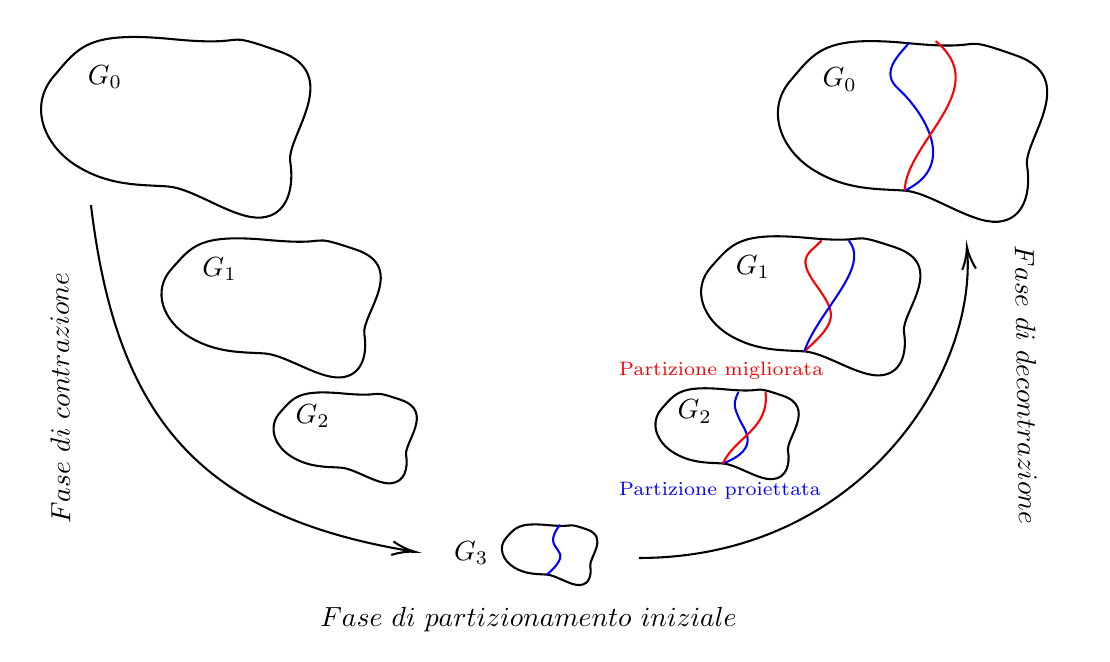
\begin{tikzpicture}[x=0.75pt,y=0.75pt,yscale=-1,xscale=1]
%uncomment if require: \path (0,301); %set diagram left start at 0, and has height of 301

%Shape: Polygon Curved [id:ds5681990127641572]
\draw   (13,23) .. controls (25,9) and (29,1) .. (70,5) .. controls (111,9) and (91,0) .. (122,11) .. controls (153,22) and (125.09,51.89) .. (127,64) .. controls (128.91,76.11) and (126,90) .. (113,91) .. controls (100,92) and (80.66,76.9) .. (68,76) .. controls (55.34,75.1) and (40,76) .. (24,66) .. controls (8,56) and (1,37) .. (13,23) -- cycle ;
%Shape: Polygon Curved [id:ds5791880784550985]
\draw   (69.88,115.65) .. controls (79.65,104.87) and (82.9,98.71) .. (116.29,101.79) .. controls (149.67,104.87) and (133.38,97.94) .. (158.63,106.41) .. controls (183.87,114.88) and (161.14,137.9) .. (162.7,147.22) .. controls (164.25,156.55) and (161.88,167.24) .. (151.3,168.01) .. controls (140.71,168.78) and (124.96,157.16) .. (114.66,156.46) .. controls (104.35,155.77) and (91.86,156.46) .. (78.83,148.76) .. controls (65.81,141.06) and (60.11,126.43) .. (69.88,115.65) -- cycle ;
%Shape: Polygon Curved [id:ds8471099289598505]
\draw   (122.17,184.81) .. controls (128.56,177.76) and (130.68,173.74) .. (152.5,175.75) .. controls (174.32,177.76) and (163.67,173.23) .. (180.17,178.77) .. controls (196.67,184.3) and (181.81,199.34) .. (182.83,205.44) .. controls (183.85,211.53) and (182.3,218.52) .. (175.38,219.02) .. controls (168.46,219.53) and (158.17,211.93) .. (151.44,211.48) .. controls (144.7,211.02) and (136.54,211.48) .. (128.02,206.44) .. controls (119.51,201.41) and (115.79,191.85) .. (122.17,184.81) -- cycle ;
%Shape: Polygon Curved [id:ds042557391147138635]
\draw   (231.1,245.21) .. controls (235.36,240.51) and (236.78,237.83) .. (251.33,239.17) .. controls (265.87,240.51) and (258.78,237.49) .. (269.78,241.19) .. controls (280.78,244.88) and (270.87,254.91) .. (271.55,258.97) .. controls (272.23,263.04) and (271.2,267.7) .. (266.58,268.03) .. controls (261.97,268.37) and (255.11,263.3) .. (250.62,263) .. controls (246.13,262.69) and (240.68,263) .. (235,259.64) .. controls (229.32,256.29) and (226.84,249.91) .. (231.1,245.21) -- cycle ;
%Shape: Polygon Curved [id:ds19971791116540039]
\draw   (368,25) .. controls (380,11) and (384,3) .. (425,7) .. controls (466,11) and (446,2) .. (477,13) .. controls (508,24) and (480.09,53.89) .. (482,66) .. controls (483.91,78.11) and (481,92) .. (468,93) .. controls (455,94) and (435.66,78.9) .. (423,78) .. controls (410.34,77.1) and (395,78) .. (379,68) .. controls (363,58) and (356,39) .. (368,25) -- cycle ;
%Shape: Polygon Curved [id:ds6697871941207159]
\draw   (329.88,114.65) .. controls (339.65,103.87) and (342.9,97.71) .. (376.29,100.79) .. controls (409.67,103.87) and (393.38,96.94) .. (418.63,105.41) .. controls (443.87,113.88) and (421.14,136.9) .. (422.7,146.22) .. controls (424.25,155.55) and (421.88,166.24) .. (411.3,167.01) .. controls (400.71,167.78) and (384.96,156.16) .. (374.66,155.46) .. controls (364.35,154.77) and (351.86,155.46) .. (338.83,147.76) .. controls (325.81,140.06) and (320.11,125.43) .. (329.88,114.65) -- cycle ;
%Shape: Polygon Curved [id:ds6317966254041107]
\draw   (306.17,182.81) .. controls (312.56,175.76) and (314.68,171.74) .. (336.5,173.75) .. controls (358.32,175.76) and (347.67,171.23) .. (364.17,176.77) .. controls (380.67,182.3) and (365.81,197.34) .. (366.83,203.44) .. controls (367.85,209.53) and (366.3,216.52) .. (359.38,217.02) .. controls (352.46,217.53) and (342.17,209.93) .. (335.44,209.48) .. controls (328.7,209.02) and (320.54,209.48) .. (312.02,204.44) .. controls (303.51,199.41) and (299.79,189.85) .. (306.17,182.81) -- cycle ;
%Curve Lines [id:da4556621139317687]
\draw [color={rgb, 255:red, 0; green, 0; blue, 255 }  ,draw opacity=1 ]   (250.62,263) .. controls (267,249) and (246,253) .. (257,239) ;
%Curve Lines [id:da3153745771749539]
\draw [color={rgb, 255:red, 0; green, 0; blue, 255 }  ,draw opacity=1 ]   (335.44,209.48) .. controls (355,202) and (345.05,192.39) .. (343.35,188.03) .. controls (341.65,183.68) and (339.62,181.49) .. (343,175) ;
%Curve Lines [id:da24590148322887484]
\draw [color={rgb, 255:red, 255; green, 0; blue, 0 }  ,draw opacity=1 ]   (335.44,209.48) .. controls (341.44,196.48) and (358,193) .. (356,175) ;
%Curve Lines [id:da8069367964557173]
\draw [color={rgb, 255:red, 255; green, 0; blue, 0 }  ,draw opacity=1 ]   (374.66,155.46) .. controls (391.66,140.46) and (390,137) .. (380,123) .. controls (370,109) and (378,108) .. (383,102) ;
%Curve Lines [id:da030698152549456736]
\draw [color={rgb, 255:red, 0; green, 0; blue, 255 }  ,draw opacity=1 ]   (374.66,155.46) .. controls (381.66,135.46) and (407,115) .. (396,102) ;
%Curve Lines [id:da9188529841976845]
\draw [color={rgb, 255:red, 0; green, 0; blue, 255 }  ,draw opacity=1 ]   (423,78) .. controls (451,65) and (429,37) .. (420,29) .. controls (411,21) and (420,13) .. (425,7) ;
%Curve Lines [id:da500049878186364]
\draw [color={rgb, 255:red, 255; green, 0; blue, 0 }  ,draw opacity=1 ]   (423,78) .. controls (424,54) and (466,29) .. (438,6) ;
%Curve Lines [id:da5337953441131338]
\draw    (31,85) .. controls (42.94,184.5) and (80.62,234.5) .. (185.42,251.74) ;
\draw [shift={(187,252)}, rotate = 189.11] [color={rgb, 255:red, 0; green, 0; blue, 0 }  ][line width=0.75]    (10.93,-3.29) .. controls (6.95,-1.4) and (3.31,-0.3) .. (0,0) .. controls (3.31,0.3) and (6.95,1.4) .. (10.93,3.29)   ;
%Curve Lines [id:da17376352225172775]
\draw    (295,255) .. controls (400.93,255) and (457.86,166.79) .. (453.16,106.81) ;
\draw [shift={(453,105)}, rotate = 84.29] [color={rgb, 255:red, 0; green, 0; blue, 0 }  ][line width=0.75]    (10.93,-3.29) .. controls (6.95,-1.4) and (3.31,-0.3) .. (0,0) .. controls (3.31,0.3) and (6.95,1.4) .. (10.93,3.29)   ;

% Text Node
\draw (28,16.4) node [anchor=north west][inner sep=0.75pt]    {$G_{0}$};
% Text Node
\draw (83.23,108.82) node [anchor=north west][inner sep=0.75pt]    {$G_{1}$};
% Text Node
\draw (128.13,179.36) node [anchor=north west][inner sep=0.75pt]    {$G_{2}$};
% Text Node
\draw (204.41,245.38) node [anchor=north west][inner sep=0.75pt]    {$G_{3}$};
% Text Node
\draw (382,17.4) node [anchor=north west][inner sep=0.75pt]    {$G_{0}$};
% Text Node
\draw (340.23,107.82) node [anchor=north west][inner sep=0.75pt]    {$G_{1}$};
% Text Node
\draw (312.13,177.36) node [anchor=north west][inner sep=0.75pt]    {$G_{2}$};
% Text Node
\draw (10.34,240.07) node [anchor=north west][inner sep=0.75pt]  [rotate=-269.56]  {$Fase\ di\ contrazione$};
% Text Node
\draw (486.92,102.91) node [anchor=north west][inner sep=0.75pt]  [rotate=-89.15]  {$Fase\ di\ decontrazione$};
% Text Node
\draw (140,277.4) node [anchor=north west][inner sep=0.75pt]    {$Fase\ di\ partizionamento\ iniziale$};
% Text Node
\draw (284,217) node [anchor=north west][inner sep=0.75pt]   [align=left] {{\scriptsize \textcolor[rgb]{0,0,1}{Partizione proiettata}}};
% Text Node
\draw (284,159) node [anchor=north west][inner sep=0.75pt]  [font=\normalsize] [align=left] {{\scriptsize \textcolor[rgb]{1,0,0}{Partizione migliorata}}};


\end{tikzpicture}

    \caption{Schema grafico del partizionamento multilivello}
    \label{fig:multi-level-graph-partitioning}
\end{figure}

L'approccio multi-livello per la partizione di grafi si articola in tre fasi principali:
\begin{enumerate}
    \item \textbf{Fase di contrazione} (\textit{contraction/coarsening phase}):
    si crea una gerarchia di grafi riducendo iterativamente la dimensione del grafo iniziale.
    Questo viene fatto comunemente individuando e contraendo coppie di nodi adiacenti, ovvero individuando un
    sottoinsieme degli archi del grafo da contrarre, $M \subseteq E $ detti \textit{match}.
    Si noti che la scelta di contrarre coppie di nodi adiacienti porta a grafi grossolani i cui nodi rappresentano
    sottografi del grafo iniziale densamente connessi.
    In base allo specifico problema, una determinata funzione di \textit{rating} classifica gli archi individuando
    quale sottoinsieme degli archi $E$ debba essere assegnato ad $M$ affinch\`e la somma dei \textit{rating} degli in
    $M$ sia globalmente massimizzata.
    Si consideri che un nodo gi\`a contratto non pu\`o essere pi\`u coinvolto in un ulteriore \textit{matching}
    allo stesso livello della gerarchia.
    \item \textbf{Fase di partizionamento iniziale} (\textit{initial partitioning phase}): quando a seguito delle
    contazioni il grafo risulta essere di ordine abbastanza piccolo, in relazione ad un qualche threshold,
    esso pu\`o essere partizionato direttamente con algoritmi costosi, fornendo una partizione inizile sul grafo
    pi\`u grossolano della gerarchia.
    \item \textbf{Fase di decontrazione} (\textit{refinement/uncoarsening phase}), i matchings vengono iterativamente
    decontratti, e i relativi nodi vengono associati a blocchi della partizione del grafo pi\`u grossolano,
    proiettandola sul grafo pi\`u raffinato.
    Per fare in modo che la partizione al livello pi\`u grossolano tenga conto delle sotto-strutture ai livelli
    pi\`u raffinati, un algoritmo di miglioramento locale (\textit{local improvement}) ricolloca i nodi tra i
    blocchi per migliorare la dimensione del taglio o l'equilibrio delle dimensioni tra i blocchi.
\end{enumerate}





